\documentclass[table, unknownkeysallowed, 10pt]{beamer}

\usetheme{Madrid}

\usepackage[spanish]{babel}

\usepackage{lmodern}

%Para poder usar las tildes. Hay que guardar el documento en uft-8
\usepackage[utf8]{inputenc}

\usepackage{amsmath}

\usepackage{mathtools}

%Para usar columnas
\usepackage{multicol}
\usepackage{multirow}
\usepackage{booktabs}
\usepackage{listings}

\usepackage{amsmath}



\definecolor{rojoUGR}{HTML}{d53044}
\definecolor{darkgray}{HTML}{737572}
\definecolor{text}{HTML}{99a6ad}
\definecolor{lightgray}{gray}{0.95}


\definecolor{lavendergray}{rgb}{0.77, 0.76, 0.82}
\colorlet{beamer@blendedblue}{rojoUGR}

\setbeamercolor{normal text}{fg=darkgray}
\setbeamercolor{block title}{bg=darkgray}
\setbeamercolor{block body}{bg=lightgray}
%\setbeamercolor{structure}{fg=rojoUGR}
%\colorlet{beamer@blendedblue}{rojoUGR}

%Color de los bulltets

\setbeamertemplate{itemize item}[square]
\setbeamercolor{itemize item}{fg=darkgray}
\setbeamertemplate{itemize subitem}[circle]
\setbeamercolor{itemize subitem}{fg=darkgray}
\setbeamercolor{itemize subsubitem}{fg=darkgray}
\setbeamertemplate{itemize subsubitem}[square]
\setbeamercolor{enumerate item}{fg=darkgray}
\setbeamertemplate{enumerate item}[square]
\setbeamertemplate{navigation symbols}{}%remove navigation symbols

\lstset{
  language=Python,
  basicstyle=\small\ttfamily,
  numbers=left,
  numberstyle=\tiny,
  numbersep=5pt,
  tabsize=2,
  extendedchars=true,
  breaklines=true,
  keywordstyle=\color{blue},
  stringstyle=\color{red},
  xleftmargin=2em,
  framexleftmargin=2em
}


\title{Uso de modelos de lenguaje de gran tamaño (LLM) de código abierto}



\subtitle{\textit{¿Es posible hacerlo "On Premise"?}}
\author{Isaac Vidal Daza}
\institute{Apoyo a la Docencia \newline Centro de Servicios de Informática y Redes de Comunicaciones \newline Universidad de Granada}
\date{28-05-2024}

% logo of my university


\titlegraphic{
   
\includegraphics[width=4cm,align=c]{imagenes/logoCSIRCDef.png}
}


%
\setbeamertemplate{footline}[text line]{FORPAS 2021}

\setbeamertemplate{footline}{%
        \hspace{0.5cm}%
        \vspace{0.2cm}%
        
\includegraphics[align=r, height=0.8cm]{imagenes/nuevoPollo2.png}%
        \hfill%
        \textit{GGTT RedIRIS - DOCENCIA-NET 2024}
        \usebeamercolor[fg]{page number in head/foot}%
        \usebeamerfont{page number in head/foot}%
        \insertframenumber\,/\,\inserttotalframenumber\kern1em%
 }

% Listing
%Para incluir código fuente
\usepackage{listings}
\lstset{ 
     basicstyle=\scriptsize\ttfamily, frame=single, columns=fullflexible,
     breaklines=true, showtabs=false, upquote=true, showstringspaces=false,
      keywordstyle=\color{blue}, numberstyle=\tiny\color{darkgray}
}

\begin{document}

\begin{frame}
    %\titlepage
    \maketitle
\end{frame}
%

%
%Sección Introducción




\begin{frame}{Teaching Support Department}
    \begin{block}{\centering Members}
        \begin{columns}
            \begin{column}{0.5\linewidth}

                \begin{itemize}
                    \item Francisco Romera Juárez. (Head)
                    \item Fernando López Álvarez.
                    \item José Guerrero Peregrina.
                    \item Antonio Cano Ruano.
                \end{itemize}

            \end{column}
            \begin{column}{0.5\linewidth}
                \begin{itemize}
                    \item Rodrigo González Gálvez.
                    \item Domingo Baca Ruíz.
                    \item Leire Melchor López.
                    \item Isaac Vidal Daza.
                \end{itemize}
            \end{column}
        \end{columns}
    \end{block}
\end{frame}


\begin{frame}{Teaching Support Department}

    \begin{columns}[T]
        \begin{column}{0.9\linewidth}
            \begin{block}{Services}
                \begin{itemize}
                    \item Computers Classrooms Management.
                    \item Software Deployment.
                    \item Virtual Desktop Infrastructure.
                    \item Microsoft 365 Management.
                    \item Systems and Services Deployment.
                \end{itemize}

            \end{block}
        \end{column}
    \end{columns}


    \begin{columns}[T]
        \begin{column}{0.5\linewidth}
            \begin{block}{Inventory}
                \begin{itemize}
                    \item 25 Faculties (Ceuta y Melilla).
                    \item 128 Computers Classrooms.
                    \item 3418 PC's.
                    \item 200 Virtual Desktops.
                \end{itemize}
            \end{block}
        \end{column}
        \begin{column}{0.4\linewidth}
            \begin{block}{Users}
                \begin{itemize}
                    \item ~53000 Students.
                    \item ~3600 Teaching Staff.
                    \item ~2200 Administration Staff.
                \end{itemize}
            \end{block}
        \end{column}
    \end{columns}

\end{frame}

\begin{frame}{Inteligencia Artificial (según los "Mass Media")}

    \begin{center}
        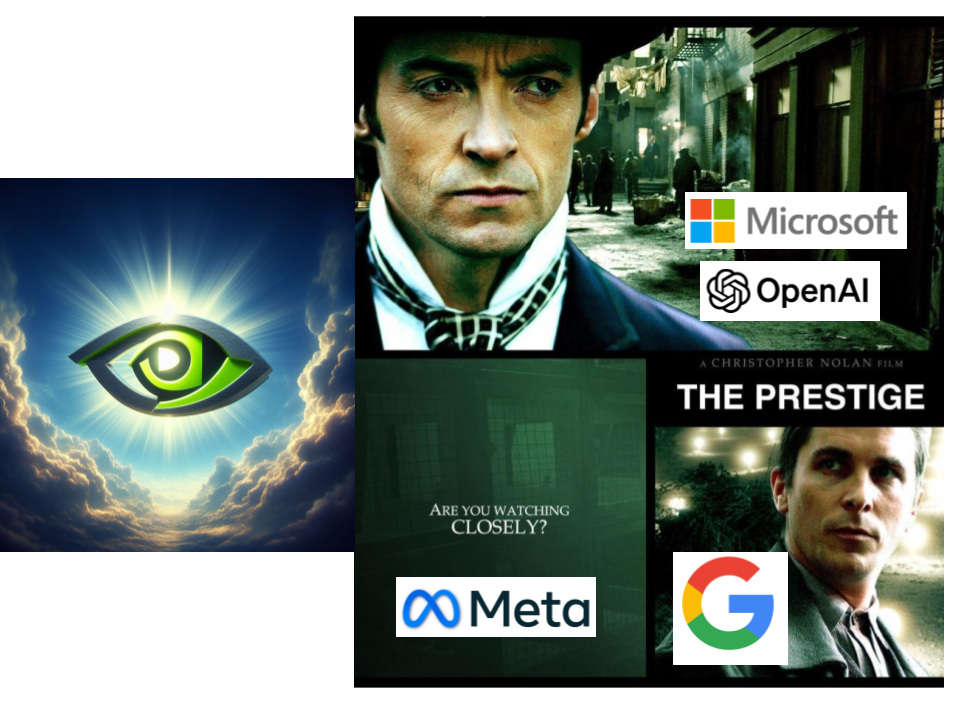
\includegraphics[width=9cm]{imagenes/final_trick.png}
    \end{center}

\end{frame}

\begin{frame}{Modelos de Lenguaje}

    \begin{block}{Lámpara Mágica}
        \begin{center}
            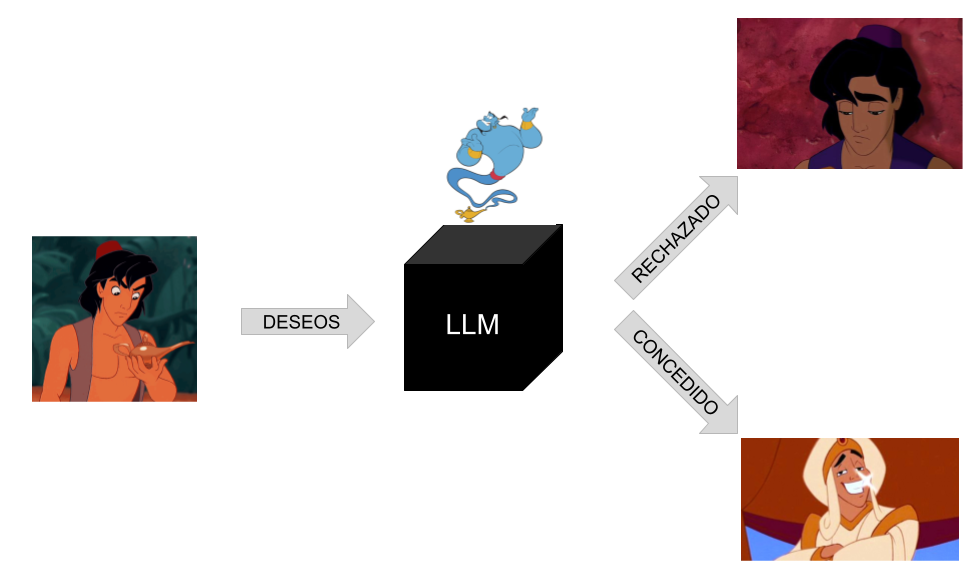
\includegraphics[width=10cm]{imagenes/llm-blacbox.png}
        \end{center}
    \end{block}

\end{frame}

\begin{frame}{Modelos de Lenguaje}

    \begin{block}{Instrucciones Precisas}
        \begin{center}
            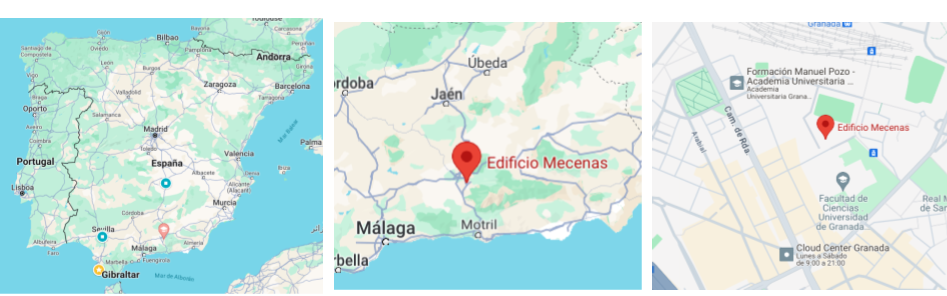
\includegraphics[width=11cm]{imagenes/prompts.png}
        \end{center}
    \end{block}


\end{frame}

\begin{frame}{¿Cómo pasar de Espectador a Ilusionista?}

    \begin{block}{Utilizando modelos LLM Open Source}
        \begin{itemize}
            \item Llama3*
            \item Mistral
        \end{itemize}
    \end{block}
    \begin{block}{¿Dónde se encuentran?}
        \begin{itemize}
            \item https://huggingface.co/
            \item https://mistral.ai/
        \end{itemize}
    \end{block}

    \begin{block}{¿Dónde ejecutan?}
        \begin{itemize}
            \item On Premise
            \item Nube
        \end{itemize}
    \end{block}

\end{frame}

\begin{frame}{¿Cómo ejecutarlos? CPUs y GPUs}

        \begin{center}
            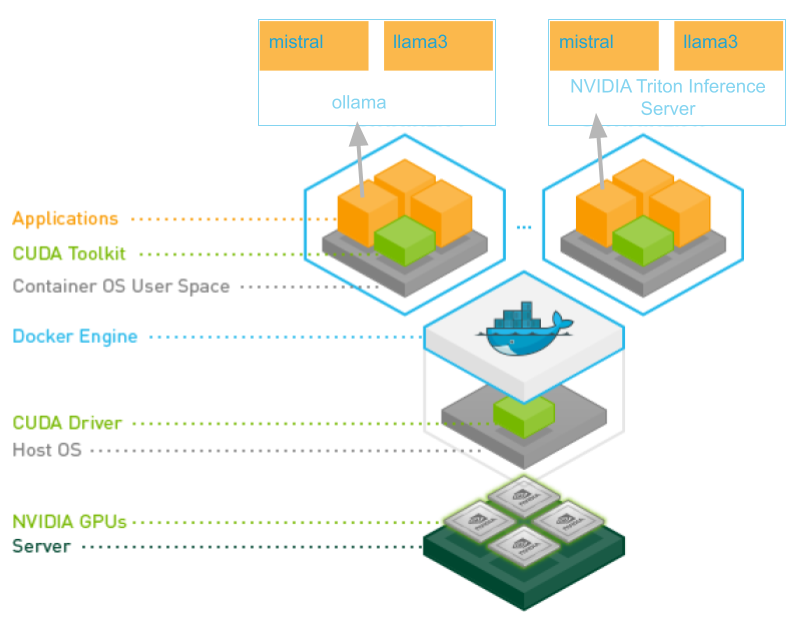
\includegraphics[width=9cm]{imagenes/docker.png}
        \end{center}

\end{frame}


\begin{frame}[fragile]{Interfaz Gráfica (unas 40 líneas de código)}

    \begin{lstlisting}[language=Python, caption=Código usando el framework Chainlit]
        @cl.on_chat_start
        async def on_chat_start():
            model = Ollama(base_url="http://localhost:11434", model="llama3")
            prompt = ChatPromptTemplate.from_messages(
                [
                    (
                        "system",
                            "You are a helpful assistant. You must always respond to Spanish questions if you receive a question in any other language. "
                    ),
                    ("human", "{question}"),
                ]
            )
            runnable = prompt | model | StrOutputParser()
            cl.user_session.set("runnable", runnable)
    \end{lstlisting}
\end{frame}

\begin{frame}[fragile]{Interfaz Gráfica (unas 40 líneas de código)}
    \begin{lstlisting}[language=Python, caption=Código usando el framework Chainlit]
        @cl.on_message
        async def on_message(message: cl.Message):
            runnable = cl.user_session.get("runnable")  # type: Runnable
        
            msg = cl.Message(content="")
        
            async for chunk in runnable.astream(
                {"question": message.content},
                config=RunnableConfig(callbacks=[cl.LangchainCallbackHandler()]),
            ):
                await msg.stream_token(chunk)
        
            await msg.send()
    \end{lstlisting}
\end{frame}

\begin{frame}{Resultado 40 líneas de código}
    \begin{block}{Asistente Personalizado}
    \begin{center}
        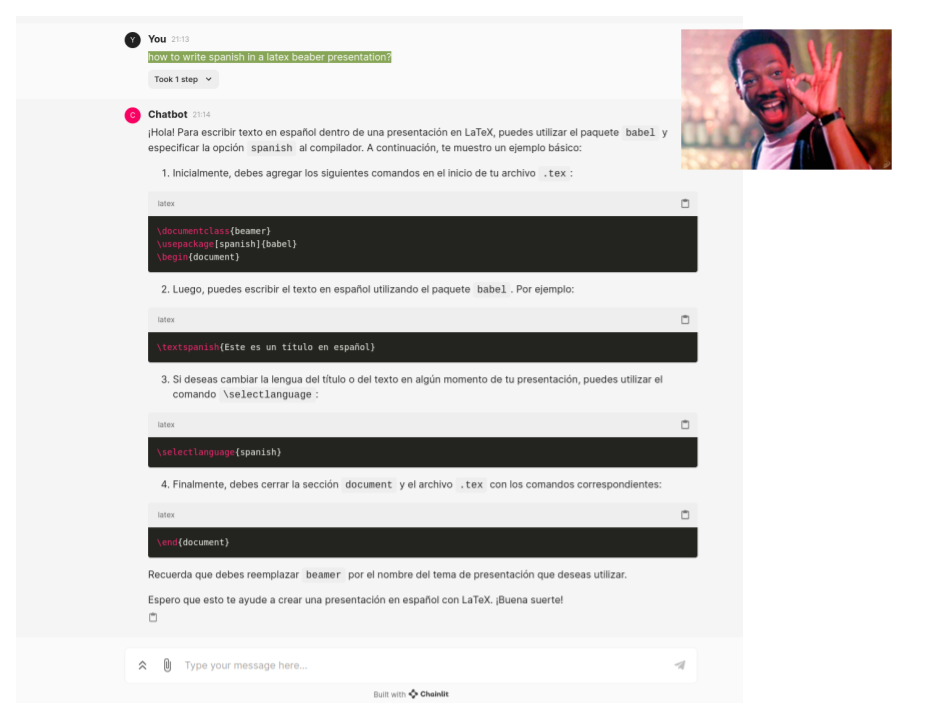
\includegraphics[width=9cm]{imagenes/chainlit.png}
    \end{center}
\end{block}

\end{frame}

\begin{frame}{Resultado 40 líneas de código}
    \begin{block}{Asistente Personalizado}
    \begin{center}
        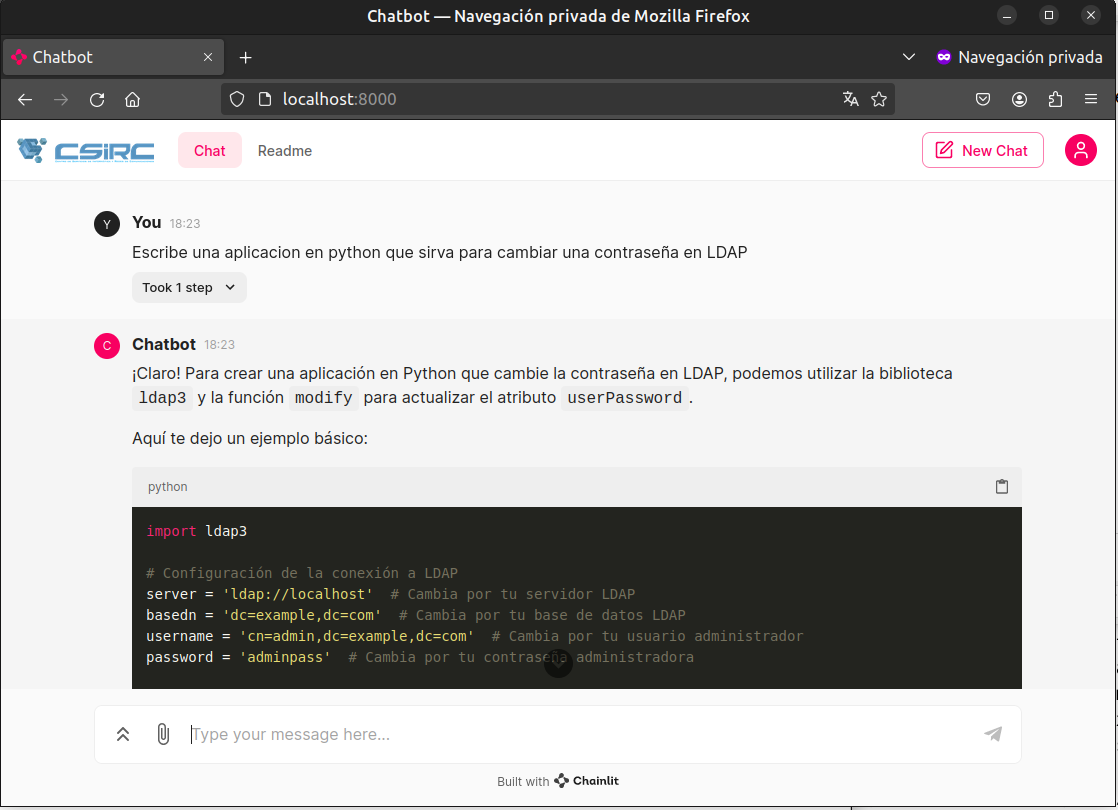
\includegraphics[width=9cm]{imagenes/chainlit1.png}
    \end{center}
\end{block}
\end{frame}

\begin{frame}{Resultado 40 líneas de código}
    \begin{block}{Asistente Personalizado}
    \begin{center}
        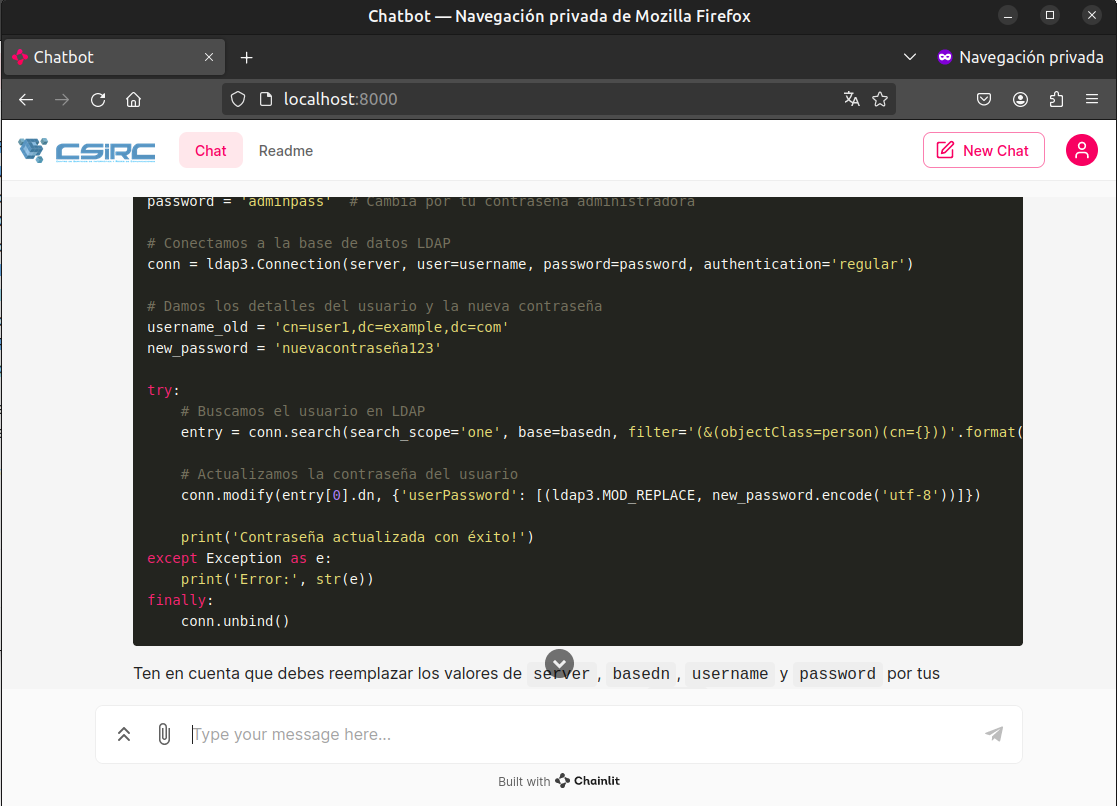
\includegraphics[width=9cm]{imagenes/chainlit2.png}
    \end{center}
\end{block}
\end{frame}

\begin{frame}{¿Puede tener memoria nuestro Asistente IA?}
    \begin{block}{¿Base de Datos SQL?}
    \begin{center}
        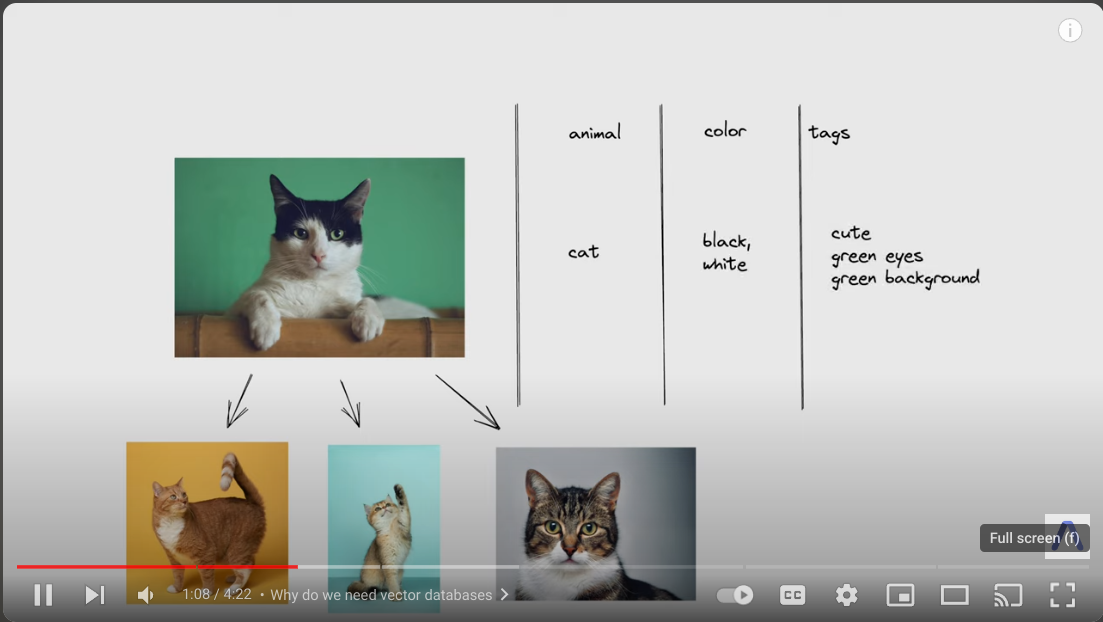
\includegraphics[width=9cm]{imagenes/vectorsql.png}
        \footnotetext{\small \href{https://www.youtube.com/watch?v=dN0lsF2cvm4}{https://www.youtube.com/watch?v=dN0lsF2cvm4}}
    \end{center}
\end{block}
\end{frame}

\begin{frame}{¿Puede tener memoria nuestro Asistente IA?}
    \begin{block}{Bases de Datos Vectoriales}
    \begin{center}
        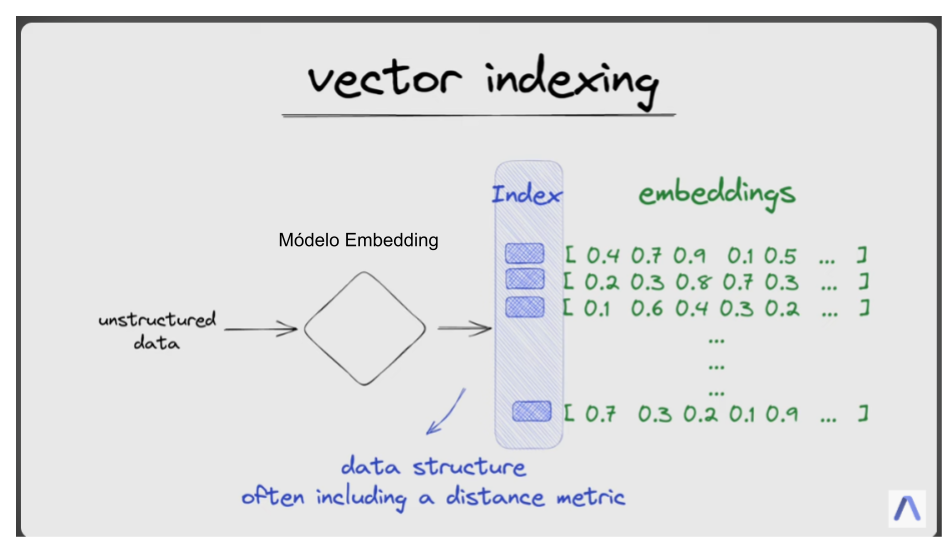
\includegraphics[width=9cm]{imagenes/vectorDB.png}
        \footnotetext{\small \href{https://www.youtube.com/watch?v=dN0lsF2cvm4}{https://www.youtube.com/watch?v=dN0lsF2cvm4}}
    \end{center}
\end{block}
\end{frame}

\begin{frame}{¿Puede tener memoria nuestro Asistente IA?}
    \begin{block}{Bases de Datos Vectoriales}
    \begin{center}
        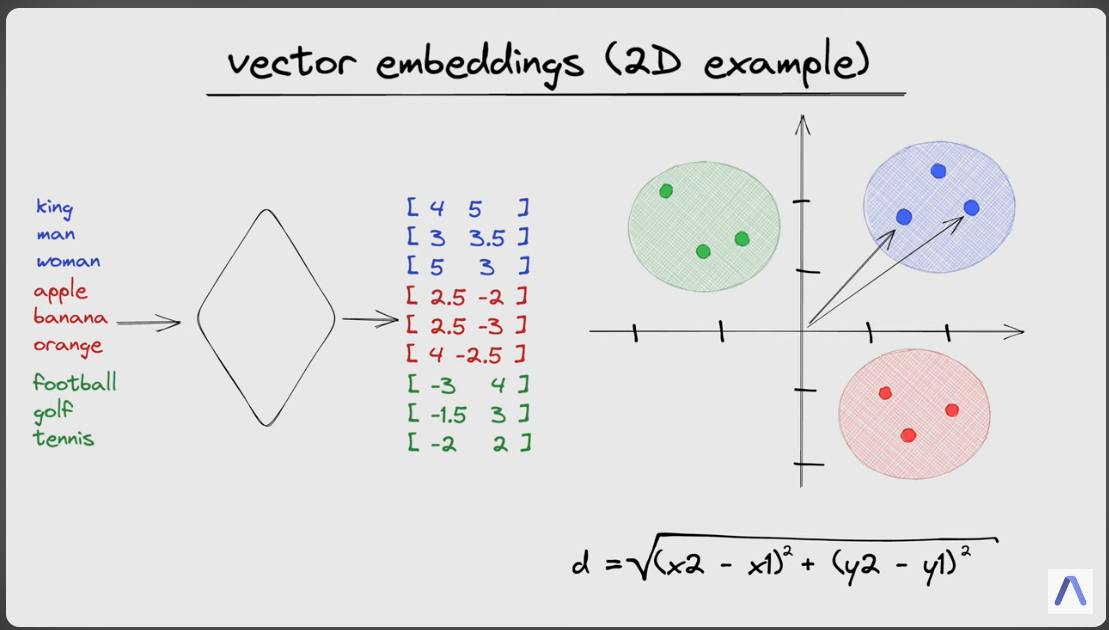
\includegraphics[width=9cm]{imagenes/vectorDB_graph.png}
        \footnotetext{\small \href{https://www.youtube.com/watch?v=dN0lsF2cvm4}{https://www.youtube.com/watch?v=dN0lsF2cvm4}}
    \end{center}
\end{block}
\end{frame}

\begin{frame}{¿Puede tener memoria nuestro Asistente IA?}

    \begin{block}{Bases de Datos Vectoriales}
    \begin{center}
        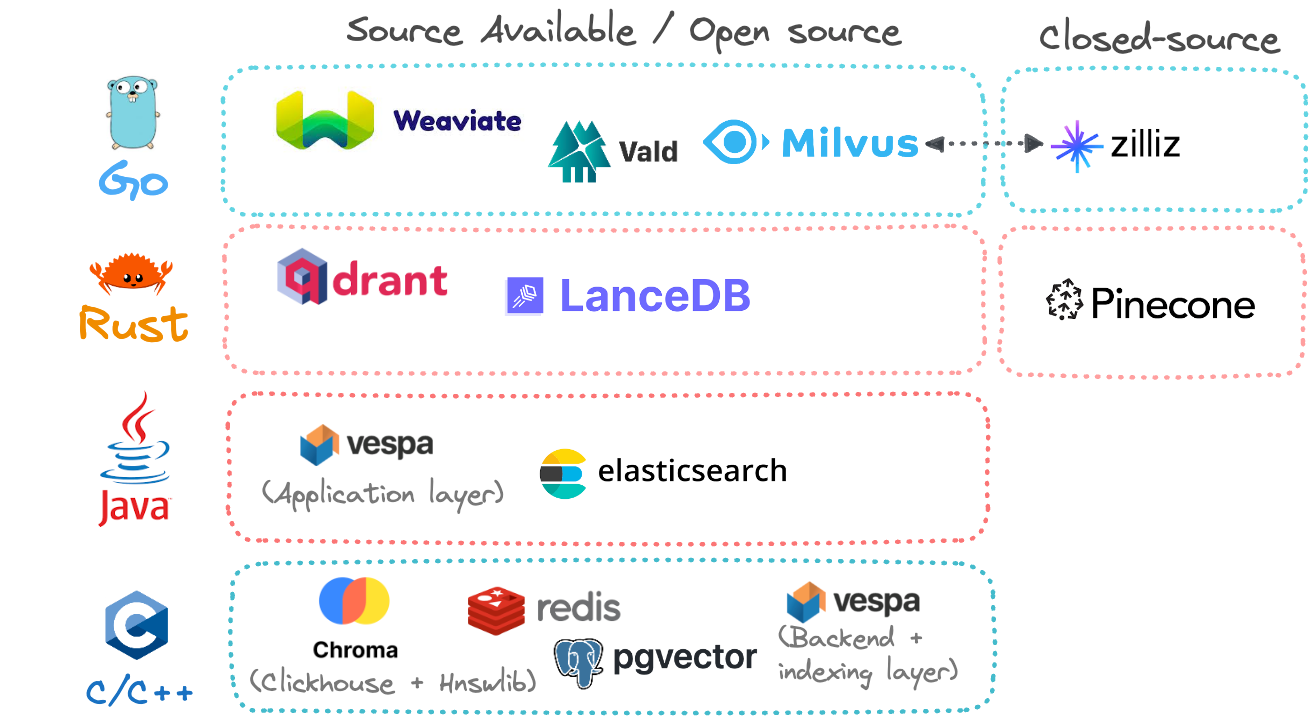
\includegraphics[width=9cm]{imagenes/tiposVectorDB.png}
        \footnotetext{\small \href{https://thedataquarry.com/posts/vector-db-1/}{https://thedataquarry.com/posts/vector-db-1/}}
    \end{center}
\end{block}
\end{frame}

\begin{frame}{LLMs y BD Vectoriales: Retrieval-Augmented Generation}
    \begin{block}{Frameworks LLM: Langchain y/o LlamaIndex}
    \begin{center}
        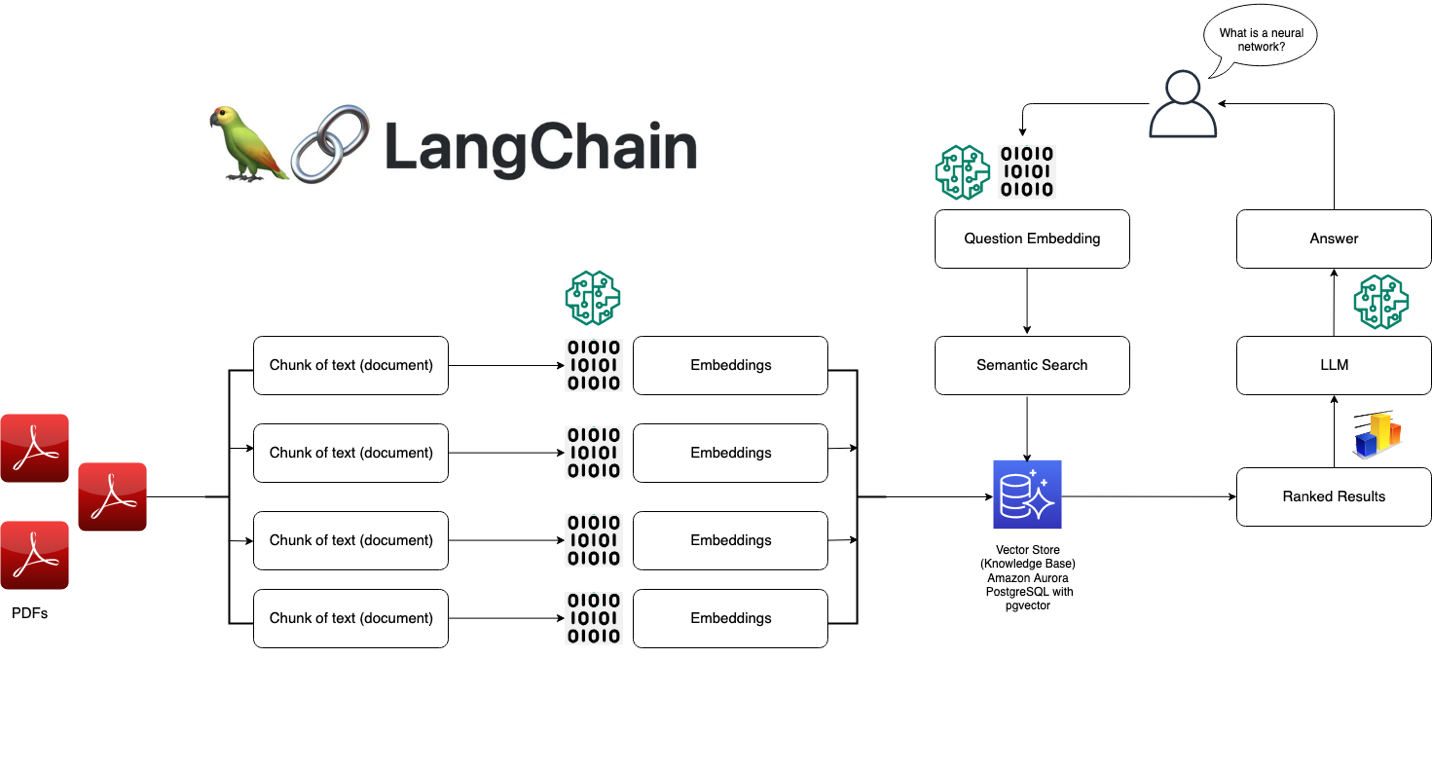
\includegraphics[width=10cm]{imagenes/langchain.png}
        \footnotetext{\small \href{https://www.langchain.com/langchain}{https://www.langchain.com/langchain}}
    \end{center}
\end{block}
\end{frame}

\begin{frame}{Agentes}
    \begin{center}
        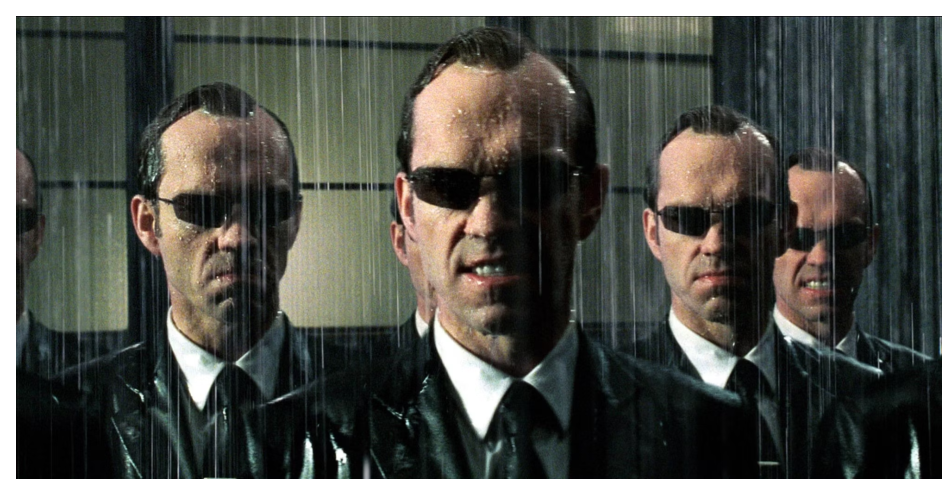
\includegraphics[width=10cm]{imagenes/agentSmith.png}
    \end{center}

\end{frame}

\begin{frame}{Framework Autogen}
    \begin{center}
        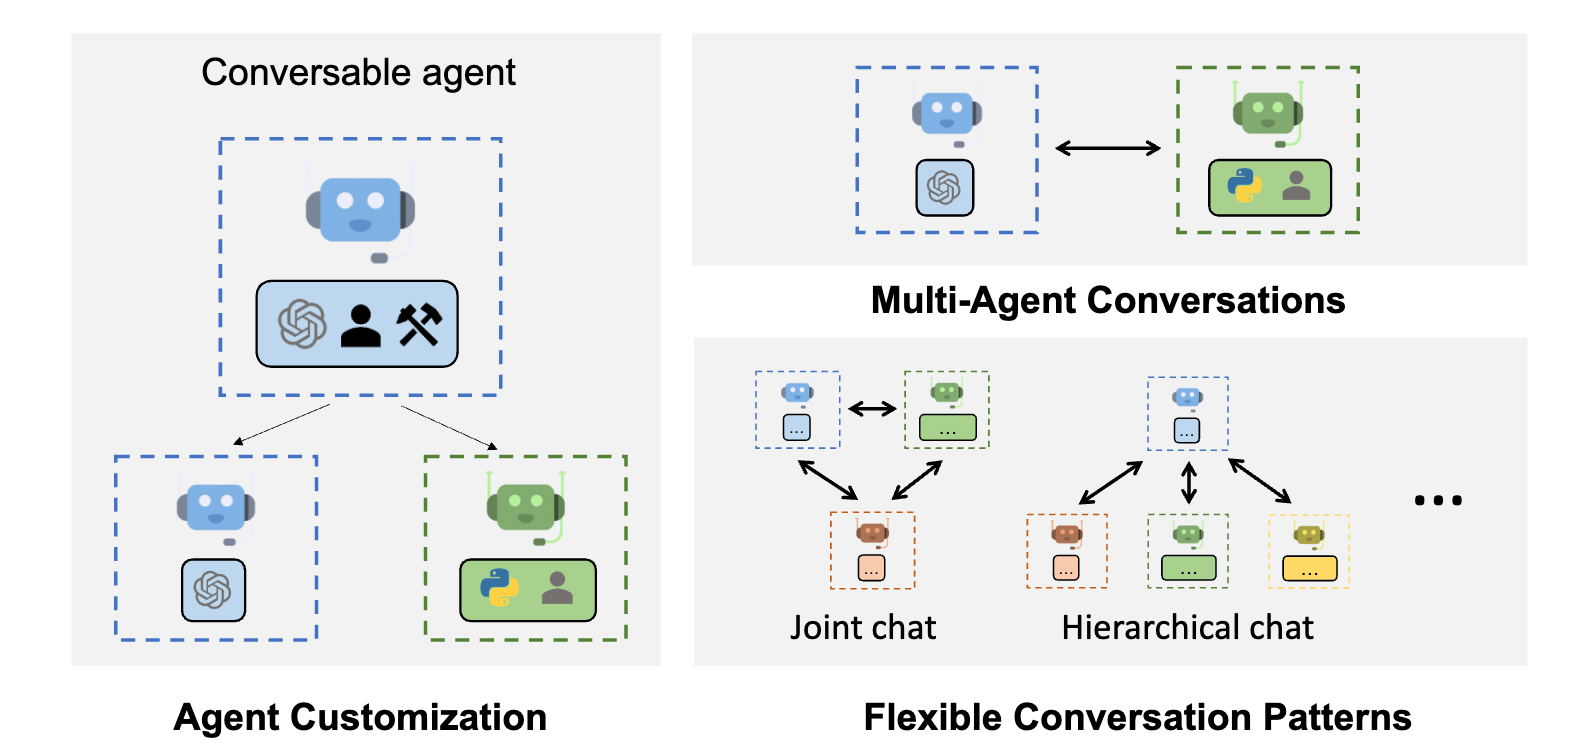
\includegraphics[width=10cm]{imagenes/autogen.png}
    \end{center}
    \footnotetext{\small \href{https://github.com/microsoft/autogen}{https://github.com/microsoft/autogen}}
\end{frame}

\begin{frame}{Preguntas}
    \begin{block}{Presentación y Código}
    \begin{center}
        \href{https://github.com/isvida/2024-RedIris}{https://github.com/isvida/2024-RedIris}
    \end{center}
\end{block}
\end{frame}




\end{document}